\documentclass[10pt]{article}

\usepackage[top=0.4in, bottom=0.4in, left=0.6in, right=0.6in]{geometry}
\usepackage{tikz}
\usetikzlibrary{positioning}
\usepackage{enumitem}
\usepackage{graphicx}
\usepackage{tgheros}
\renewcommand*{\familydefault}{\sfdefault}

\setlength{\parskip}{0pt}

% Change this value to resize the grade circle on the quiz header.
\newlength{\gradeCircleRadius}
\setlength{\gradeCircleRadius}{0.35in}

% Set this to the letter identifying this quiz version (e.g. A, B).
\newcommand{\quizVersion}{B}

% Reference diagrams of the USB and CAN frame structures, shown below each
% waveform (not to scale) to help students locate fields in the questions.
\newcommand{\usbFrameDiagram}{%
\begin{center}
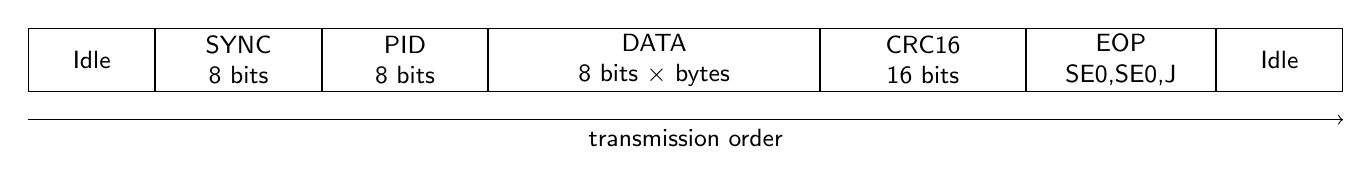
\begin{tikzpicture}[field/.style={draw, minimum height=0.8cm, align=center, font=\small, inner sep=2pt}]
\node[field, minimum width=1.6cm] (idle1) {Idle};
\node[field, minimum width=2.1cm, right=0pt of idle1] (sync) {SYNC\\8 bits};
\node[field, minimum width=2.1cm, right=0pt of sync] (pid) {PID\\8 bits};
\node[field, minimum width=4.2cm, right=0pt of pid] (data) {DATA\\8 bits $\times$ bytes};
\node[field, minimum width=2.6cm, right=0pt of data] (crc) {CRC16\\16 bits};
\node[field, minimum width=2.4cm, right=0pt of crc] (eop) {EOP\\SE0,SE0,J};
\node[field, minimum width=1.6cm, right=0pt of eop] (idle2) {Idle};
\draw[->] ([yshift=-0.35cm]idle1.south west) -- node[below, font=\small]{transmission order} ([yshift=-0.35cm]idle2.south east);
\end{tikzpicture}
\end{center}}

\newcommand{\canFrameDiagram}{%
\begin{center}
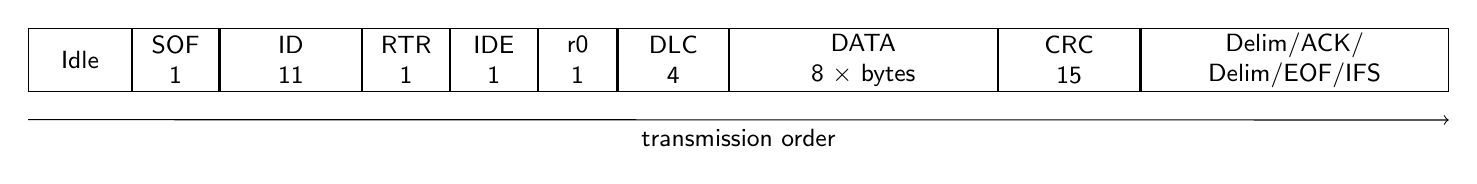
\begin{tikzpicture}[field/.style={draw, minimum height=0.8cm, align=center, font=\small, inner sep=1.5pt}]
\node[field, minimum width=1.3cm] (idle1) {Idle};
\node[field, minimum width=1.1cm, right=0pt of idle1] (sof) {SOF\\1};
\node[field, minimum width=1.8cm, right=0pt of sof] (id) {ID\\11};
\node[field, minimum width=1.1cm, right=0pt of id] (rtr) {RTR\\1};
\node[field, minimum width=1.1cm, right=0pt of rtr] (ide) {IDE\\1};
\node[field, minimum width=1.0cm, right=0pt of ide] (r0) {r0\\1};
\node[field, minimum width=1.4cm, right=0pt of r0] (dlc) {DLC\\4};
\node[field, minimum width=3.4cm, right=0pt of dlc] (data) {DATA\\8 $\times$ bytes};
\node[field, minimum width=1.8cm, right=0pt of data] (crc) {CRC\\15};
\node[field, minimum width=3.9cm, right=0pt of crc] (tail) {Delim/ACK/\\Delim/EOF/IFS};
\draw[->] ([yshift=-0.35cm]idle1.south west) -- node[below, font=\small]{transmission order} ([yshift=-0.35cm]tail.south east);
\end{tikzpicture}
\end{center}}

\pagestyle{empty}

\begin{document}

\noindent
\begin{minipage}[t]{\dimexpr\textwidth-2\gradeCircleRadius-0.5in\relax}
    {\large\textbf{ECGR 4101/5101 --- Advanced Embedded Systems}}\par
    \textbf{Quiz 1: USB and CAN Bus --- Version \quizVersion}\\[8pt]
    Name: \makebox[2in]{\hrulefill} \quad Date: \makebox[1.1in]{\hrulefill}
\end{minipage}%
\hfill
\raisebox{0.15in}{%
\begin{minipage}[t]{\dimexpr 2\gradeCircleRadius+0.2in\relax}
    \centering
    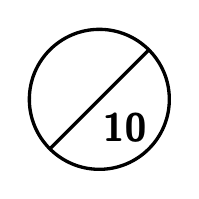
\begin{tikzpicture}[baseline=(circtop.base)]
        \coordinate (circtop) at (0,\gradeCircleRadius);
        \draw[very thick] (0,0) circle (\gradeCircleRadius);
        \draw[very thick] ({\gradeCircleRadius*cos(225)},{\gradeCircleRadius*sin(225)}) -- ({\gradeCircleRadius*cos(45)},{\gradeCircleRadius*sin(45)});
        \node at ({0.36*\gradeCircleRadius},{-0.4*\gradeCircleRadius}) {\Large\textbf{10}};
    \end{tikzpicture}
\end{minipage}}

\vspace{0.05in}
\textit{For each question, circle the letter of the correct answer.}

\vspace{0.05in}

\setlist[enumerate]{topsep=0pt, itemsep=2pt, parsep=0pt}

\begin{enumerate}[label=\textbf{\arabic*.}, leftmargin=*, itemsep=4pt]

\item \textbf{(5 points)} The figure below is a capture of the D+ and D- lines during a single USB data packet. The numbers along the top count the bit times, and each dotted line marks the boundary between two bit times.

\begin{center}
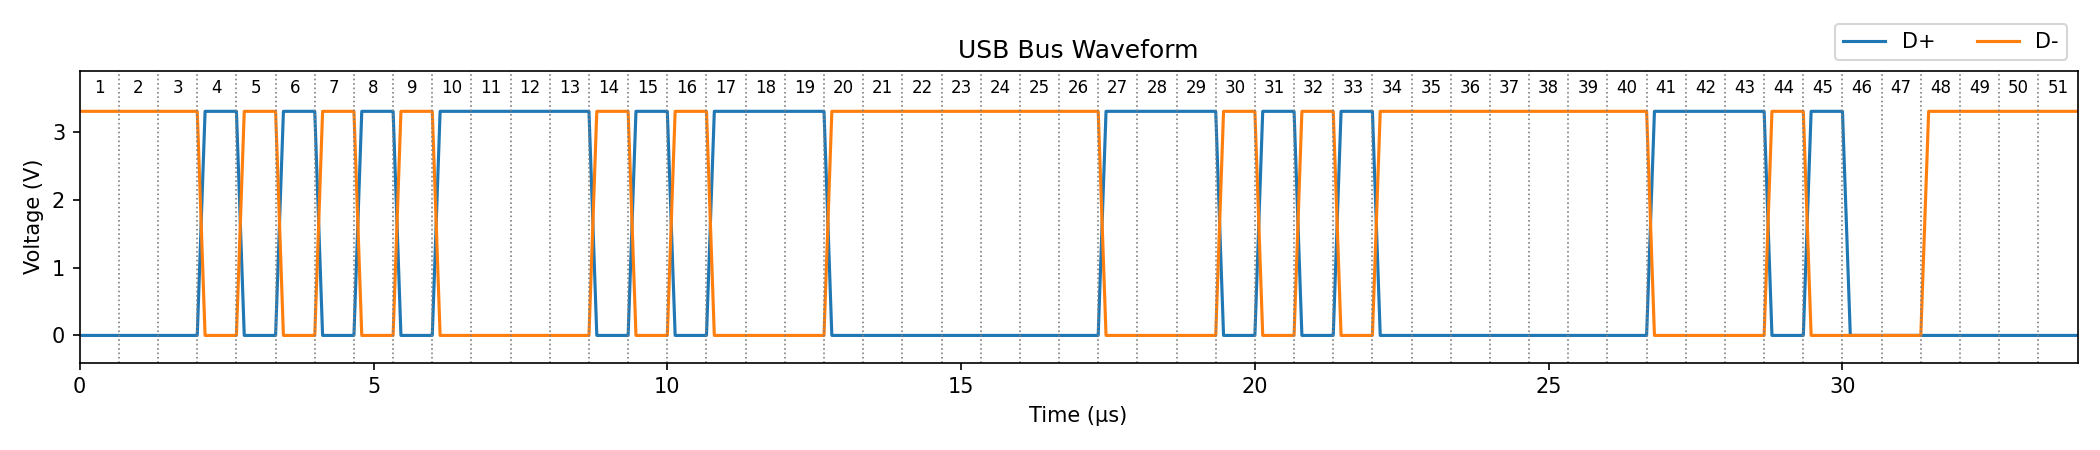
\includegraphics[width=\linewidth]{usb_waveform.png}
\end{center}
\vspace{-12pt}
\usbFrameDiagram
\vspace{-10pt}

\begin{enumerate}[label=(\alph*), leftmargin=*, itemsep=3pt]
\item \textbf{(2 points)} Based on the bit time shown in the waveform above, is this a low-speed or full-speed USB packet?

\centerline{\textbf{(A)} Full-speed (12 Mbit/s) \qquad \textbf{(B)} High-speed (480 Mbit/s)}
\centerline{\textbf{(C)} Low-speed (1.5 Mbit/s) \qquad \textbf{(D)} Cannot be determined}

\item \textbf{(2 points)} Which of the following is the correct SYNC field bit pattern (LSB first, as transmitted on the bus)?

\centerline{\textbf{(A)} 11111110 \qquad \textbf{(B)} 01111111 \qquad \textbf{(C)} 00000001 \qquad \textbf{(D)} 10000000}

\item \textbf{(1 point)} Which bit time(s) contain a bit-stuffing bit?

\centerline{\textbf{(A)} bit 41 only \qquad \textbf{(B)} bit 27 only \qquad \textbf{(C)} bits 27 and 41 \qquad \textbf{(D)} none}
\end{enumerate}

\item \textbf{(5 points)} The figure below is a capture of the CAN\_H and CAN\_L lines during a single \textbf{standard frame} (11-bit identifier) CAN data frame.

\begin{center}
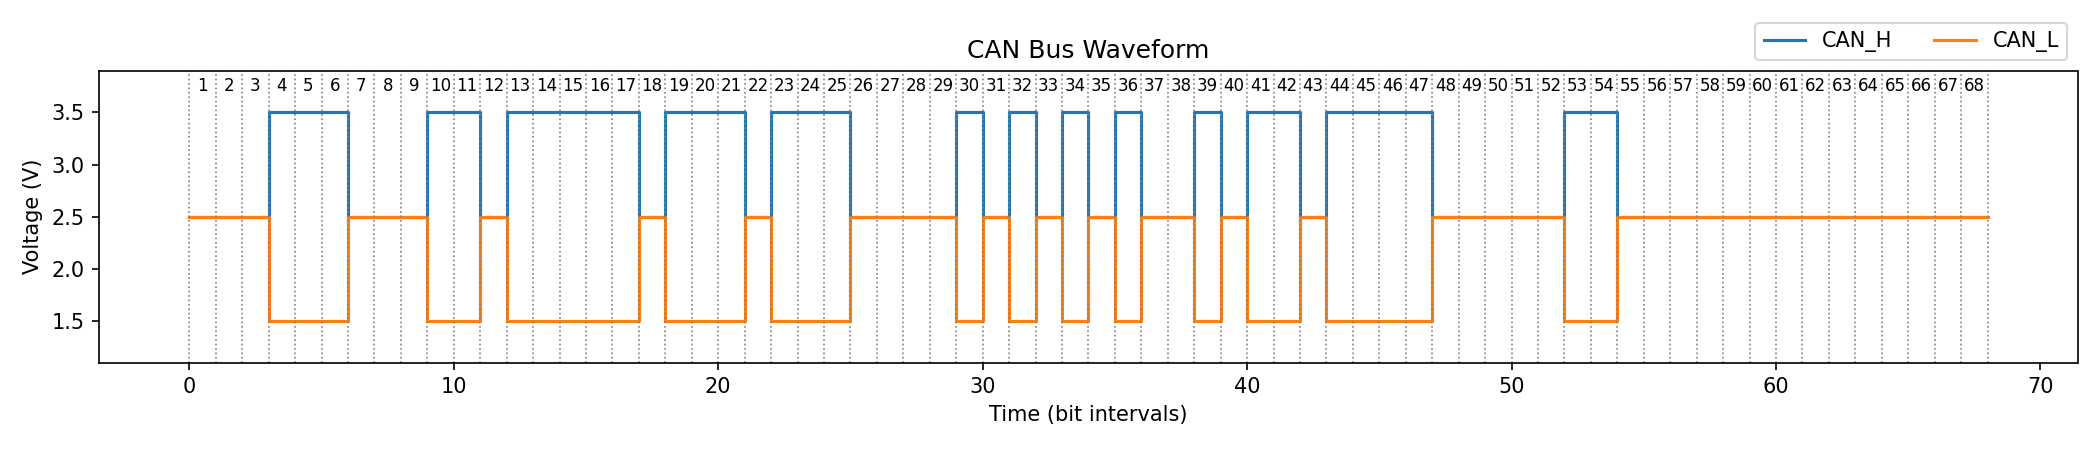
\includegraphics[width=\linewidth]{can_waveform.png}
\end{center}
\vspace{-12pt}
\canFrameDiagram
\vspace{-10pt}

\begin{enumerate}[label=(\alph*), leftmargin=*, itemsep=3pt]
\item \textbf{(1 point)} On the physical bus, a \textbf{dominant} bit corresponds to which logic level?

\centerline{\textbf{(A)} High impedance \qquad \textbf{(B)} Depends on the transmitting node \qquad \textbf{(C)} Logic 1 \qquad \textbf{(D)} Logic 0}

\item \textbf{(1 point)} Which bit time(s) contain a bit-stuffing bit?

\centerline{\textbf{(A)} bit 18 only \qquad \textbf{(B)} bit 53 only \qquad \textbf{(C)} bits 18 and 53 \qquad \textbf{(D)} none}

\item \textbf{(1 point)} How many data bytes does this frame carry?

\centerline{\textbf{(A)} 4 \qquad \textbf{(B)} 1 \qquad \textbf{(C)} 2 \qquad \textbf{(D)} 3}

\item \textbf{(1 point)} Decode the 11-bit identifier carried by this frame. Give your answer in hex.

\centerline{\textbf{(A)} 0x1A8 \qquad \textbf{(B)} 0x5C8 \qquad \textbf{(C)} 0x1C8 \qquad \textbf{(D)} 0x1C9}

\item \textbf{(1 point)} If we have two identifiers that were transmitted at the same time, which one would be placed on the bus?

\centerline{\textbf{(A)} Whichever node started transmitting first \qquad \textbf{(B)} Both are placed on the bus simultaneously}

\centerline{\textbf{(C)} The identifier with the numerically lower value \qquad \textbf{(D)} The identifier with the numerically higher value}
\end{enumerate}

\end{enumerate}

\end{document}
